\subsection{The Set of Complex Numbers}

We can define $\CC$ as follows:
\[ \CC = \{ z = ix +y | (x,y) \in \RR^2 \}. \] 
Note that $\CC$ is a commutative field, under standard addition and multiplication. Formally, addition is defined as 

\begin{exercise}
Verify that $\CC$ satisfies the definition of a commutative field. 
\end{exercise}

\subsection{Motivations: The Fundamental Theorem of Algebra}
\begin{theorem}[Fundamental Theorem of Algebra]
A polynomial $p(z) = a_nz^n + a_{n-1}z^{n-1} + \cdots + a_1z + a_0$, where $a_i \in \CC$ for all $i$ and $a_n \neq 0$, is a product of $n$ linear factors; There exist $r_1, r_2, \ldots, r_n \in \CC$ such that 
\[ p(z) = a_n\prod_{k=1}^n z-r_k. \] 
\end{theorem}
This is a fundamental result, and it can finally be proved using complex-analytic techniques. 
\begin{corollary*}
If $p(z)$ has all real coefficients, it factors into a product of linear and irreducible over $\RR$ quadratic factors. 
\end{corollary*}
As complex roots come in complex pairs, their product ($z\cdot \overline{z}$), we obtain a quadratic factor that is irreducible over $\RR$. 
\subsection{Complex Plane}
% \begin{figure}[h]
% \centering

% \begin{tikzpicture}
% \draw[thick,->] (0,0) -- (4,0);
% \draw[thick,->] (0,0) -- (0,4);
% \draw[thick,->] (0,0) -- (0,-4);

% \draw[thick, dashed, red] (0,0) -- (3,3);
% \node[label=z] (a) at (3,3);
% \filldraw[red] (a) circle (1pt);

% \draw[thick, dashed, red] (0,0) -- (3,-3);
% \node[label=$\overline{z}$] (b) at (3,-3);
% \filldraw[red] (b) circle (1pt);
% \end{tikzpicture}
% \end{figure}

$\CC$ is \emph{not} an ordered set! For $w,z \in \CC$, we cannot write $z < w$ or $w < z$. Recall that addition in the complex plane follows the \vocab{parallelogram law}. This leads to the following: 
\begin{proposition}[Triangle Inequality in Complex Plane]
For any $w,z \in \CC$, we have 
\[ |w + z| \leq |w| + |z|. \] 
\end{proposition}
\begin{proof}
We can construct a triangle using side lengths equal to the moduli, and the result follows.
\end{proof}
Visually, we have the following: 

\begin{figure}[h]
\centering

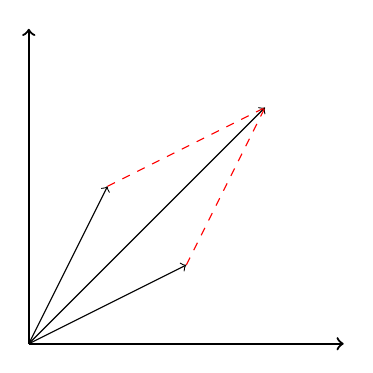
\begin{tikzpicture}
\draw[thick,->] (0,0) -- (4,0);
\draw[thick,->] (0,0) -- (0,4);

\draw[->] (0,0) -- (1,2);
\draw[->] (0,0) -- (2,1);

\draw[->] (0,0) -- (3,3);

\draw[dashed,red] (2,1) -- (3,3);


\draw[dashed,red] (1,2) -- (3,3);
\end{tikzpicture}
\end{figure}

We also have the following corollary: 
\begin{corollary}
For a polynomial $p(z) = \sum\limits_{k=0}^n a_kz^k$, where $a_i \in \CC$ for all  $i$, and $a_n \neq 0$, there exists an $R \in \RR$ such that 
\[ \left | \frac{1}{p(z)} \right | < \frac{2}{|a_n|R^n} \] for all $z$, such that $|z| > R$. 
\end{corollary}
\begin{proof}
Let 
\[ \omega = \frac{a_0}{z^n} + \frac{a_1}{z^{n-1}} + \cdots + \frac{a_{n-1}}{z}. \] 
Then $\omega z^n = a_0 + a_1z + \cdots a_{n-1}z^{n-1} = p(z) - a_nz^n$.

Note that 
\[ |\omega||z|^n = |\omega z^n| \leq |a_0| + |a_1||z| + \cdots |a_{n-1}||z|^{n-1} \] implies that 
\[ |\omega| \leq \frac{|a_0|}{|z|^n} + \frac{|a_1|}{|z|^{n-1}} + \cdots + \frac{|a_{n-1}}{|z|}. \] There exists an $R \in \RR$ such that 
\[ \max\limits_{i=0,\ldots,n-1} \left \{ \frac{|a_i|}{R^{n-i}} \right \} < \frac{|a_n|}{2n}. \] This implies that $|\omega| < \frac{|a_n|}{2}$, for all $z$ such that $|z| > R$. As $p(z) = (a_n + \omega)z^n$ for $z \neq 0$, we have 
\[ |p(z)| = |a_n + \omega||z|^n \geq ||a_n| - |\omega|||z|^n. \] Then for all $z$ such that $|z| > R$, 
\[ |p(z)| \geq \frac{a_n}{2}R^n, \] as desired. 
\end{proof}
